\chapter{\IfLanguageName{dutch}{Stand van zaken}{State of the art}}%
\label{ch:stand-van-zaken}

Een toepassing voor geautomatiseerde en gepersonaliseerde tekstvereenvoudiging van wetenschappelijke artikelen vereist een grondige literatuurstudie van de drie domeinen. Om een gepersonaliseerde tool aan te reiken, is het van cruciaal belang om de noden van de scholieren met dyslexie grondig te begrijpen. Dit kan alleen worden bereikt door middel van een gedetailleerde analyse van de literatuur die beschikbaar is op dit gebied. Bij het uitvoeren van deze literatuurstudie moet er aandacht worden besteed aan de verschillende vereenvoudigingstechnieken die momenteel ingezet worden. Door deze technieken te bestuderen, kan er een beter begrip van de mogelijkheden en beperkingen van elke techniek worden gevormd. Ten slotte moet er bij de ontwikkeling van een AI-toepassing voor tekstvereenvoudiging rekening worden gehouden met de valkuilen die vaak voorkomen bij dergelijke projecten. Door deze valkuilen te vermijden en gebruik te maken van de kennis die is opgedaan in de literatuurstudie, kan een effectieve en waardevolle tool worden ontwikkeld die aan de noden van scholieren met dyslexie voldoet.

\section{Specifieke noden van scholieren met dyslexie in de derde graad van het middelbaar onderwijs}

Deze sectie gaat in op de unieke noden en bespreken hoe mensen met dyslexie kunnen worden geholpen bij het lezen. Daarnaast worden de belemmeringen en moeilijkheden van wetenschappelijke artikelen aangekaart. Deze sectie beantwoordt de volgende twee onderzoeksvragen: 
\begin{itemize}
	\item Welke specifieke noden hebben scholieren met dyslexie van de derde graad middelbaar onderwijs bij het begrijpen van complexere teksten?
	\item Wat zijn de specifieke kenmerken van wetenschappelijke artikelen?
\end{itemize}



\subsubsection{Centraal zicht op dyslexie}

% Lezen is een essentieel onderdeel van ons dagelijks leven en speelt een belangrijke rol in onze onderlinge communicatie en begrip. Dyslexie kan het lezen moeilijker maken. Het begrijpen van de noden en hindernissen voor een scholier met dyslexie is van belang om deze doelgroep te ondersteunen en hun kwaliteit van lezen te verbeteren. 

Leesvaardigheid is geen aangeboren vaardigheid. Het aanleren van deze vaardigheid vereist een herinrichting van het brein, zoals vermeld in de onderzoeken van \textcite{Bonte2020, VanDerMeer2022}. Hoewel deze herinrichting bij sommige mensen vlot verloopt, kunnen mensen met dyslexie benadeeld worden bij dit proces. Dyslexie wordt gekenmerkt door beperkt lezen en kan het voorlezen traag, radend en letter-voor-letter maken. Een goede woordenschatontwikkeling of vaak voorlezen kan echter bescherming bieden tegen dyslexie, zoals aangegeven in de onderzoeken van \textcite{Vellutino2004, Bonte2020}. Onderzoeken halen drie verschillende diagnoses van dyslexie aan:

\begin{itemize}
	\item Fonologische dyslexie
	\item Surface dyslexia
	\item Deep dyslexia
\end{itemize}

Dezelfde onderzoeken wijzen erop dat een overlap van kenmerken over de drie types heen mogelijk is \autocite{Rello2012, Vellutino2004}. Fonologische dyslexie is de meest prevalente vorm bij scholieren met dyslexie in de derde graad van het onderwijs en vormt daarmee het focuspunt van dit onderzoek.

\subsubsection{Mogelijke drempels voor mensen met dyslexie}

Mensen met dyslexie kunnen verschillende drempels ervaren, waaronder trage woordbenoeming, hardnekkig letter-voor-letter lezen, problemen met woordherkenning en -herinnering, letter- en klankvorming, homofonische of pseudo-homofonische woordenschat en begripsproblemen \autocite{Bonte2020, RiveroContreras2021, Zhang2021}. 

\begin{table}[!ht]
	\centering
	\begin{tabular}{|l|l|}
		\hline
		Knelpunt & Omschrijving \\ \hline
		Trage woordbenoeming & Moeite hebben met het snel benoemen van woorden, vooral bij het lezen \\ \hline
		Hardnekkig letter-voor-letter lezen & Het lezen van woorden als afzonderlijke letters in plaats van als een geheel \\ \hline
		Problemen met woordherkenning en -herinnering & Moeite hebben om woorden te herkennen en te onthouden \\ \hline
		Letter- en klankvorming & Moeite hebben met het koppelen van letters aan klanken en het uitspreken van woorden \\ \hline
		Homofonische of pseudo-homofonische woordenschat & Verwarring tussen woorden die hetzelfde klinken maar anders gespeld worden, zoals "koe" en "kauw" \\ \hline
		Begripsproblemen & Moeite hebben met het begrijpen van de inhoud van een tekst \\ \hline
		Schriftelijke expressie & Moeite hebben met het schrijven van woorden en zinnen \\ \hline
	\end{tabular}
	\caption{Drempels bij fonologische dyslexie \autocite{Bonte2020, RiveroContreras2021, Zhang2021}}
	\label{tab:dyslexie-drempels}
\end{table}

\subsection{Specifieke kenmerken van wetenschappelijke artikelen}

Wetenschappelijke artikelen volgen een IMRAD-formaat\footnote{Uniform formaat voor gepubliceerde wetenschappelijke artikelen. De structuur bestaat uit vijf hoofdstukken: inleiding, methodologie, resultaten en discussie.} en worden gebruikt als leermiddel voor jongeren in het middelbaar en hoger onderwijs. 

\subsubsection{Leesgraad}

De leesbaarheid van tekst kan zowel subjectief als objectief worden beoordeeld. Subjectieve beoordelingen worden gemaakt op basis van intuïtie en inschatting van de doelgroep, terwijl teksten ook kunnen worden beoordeeld met behulp van leesbaarheidsscores. In het volgende worden de drie belangrijkste leesbaarheidsscores beschreven.

% FLESCH = zinbasis
% G FOG = tekstbasis

FLESCH is de meest prevalente leesbaarheidsscore. De ranking gebeurt als volgt:

\begin{tabular}{|c|c|c|}
	\hline
	\textbf{Score} & \textbf{Leesbaarheid} & \textbf{Niveau} \\
	\hline
	0-30 & Zeer moeilijk & Universiteit \\
	\hline
	30-50 & Moeilijk & Hoger onderwijs \\
	\hline
	50-60 & Redelijk moeilijk & Middelbare school \\
	\hline
	60-70 & Redelijk makkelijk & Basisschool \\
	\hline
	70-80 & Makkelijk & Eenvoudig \\
	\hline
	80-90 & Zeer makkelijk & Zeer eenvoudig \\
	\hline
\end{tabular}


\subsubsection{Trends rond wetenschappelijke artikelen}

De leesgraad van wetenschappelijke teksten volgt al sinds de tweede helft van de twintigste eeuw een stijgende trend \autocite{Hayes1992}. Meerdere onderzoeken in de voorbije tien jaar besluiten dat de complexe woordenschat en zinsbouw deze wetenschappelijke artikelen ontoegankelijk maken voor doelgroepen naast onderzoekers \autocite{Ball2017, PlavenSigray2017, Jones2019}. 

\textcite{PlavenSigray2017} onderzoeken de verschillende trends waarom wetenschappelijke artikelen alsmaar moeilijker worden om te lezen. Dit onderzoek brengt de relatie tussen de leesbaarheid van een abstract en het publicatiejaar in kaart. De \textit{Flesch-Reading-Ease} of FRE score werd gebruikt om de leesgraad van een wetenschappelijk artikel te beoordelen. Om te bevestigen dat de relatie tussen de complexiteit van een abstract overeenstemt met die van de volledige tekstinhoud, werden er vergelijkingen gemaakt met zes verschillende wetenschappelijke journalen. De overeenkomst tussen de leesgraad van het abstract en de overige tekstinhoud in een wetenschappelijk artikel werd eerder bevestigd door \textcite{Dronberger1975}. Dat onderzoek benadrukt dat een abstract complexer wordt geschreven, vergeleken met de andere hoofdstukken van een wetenschappelijk artikel. Op \ref{img:fre-ndc} wordt de evolutie per FRE (links) en NDC-score (rechts) getoond. Het onderzoek schat dat nu 22\% van alle wetenschappelijke artikelen gebruik maken van Engels op het niveau van een masterstudent, vergeleken met 14\% in 1960. 

\begin{figure}[H]
	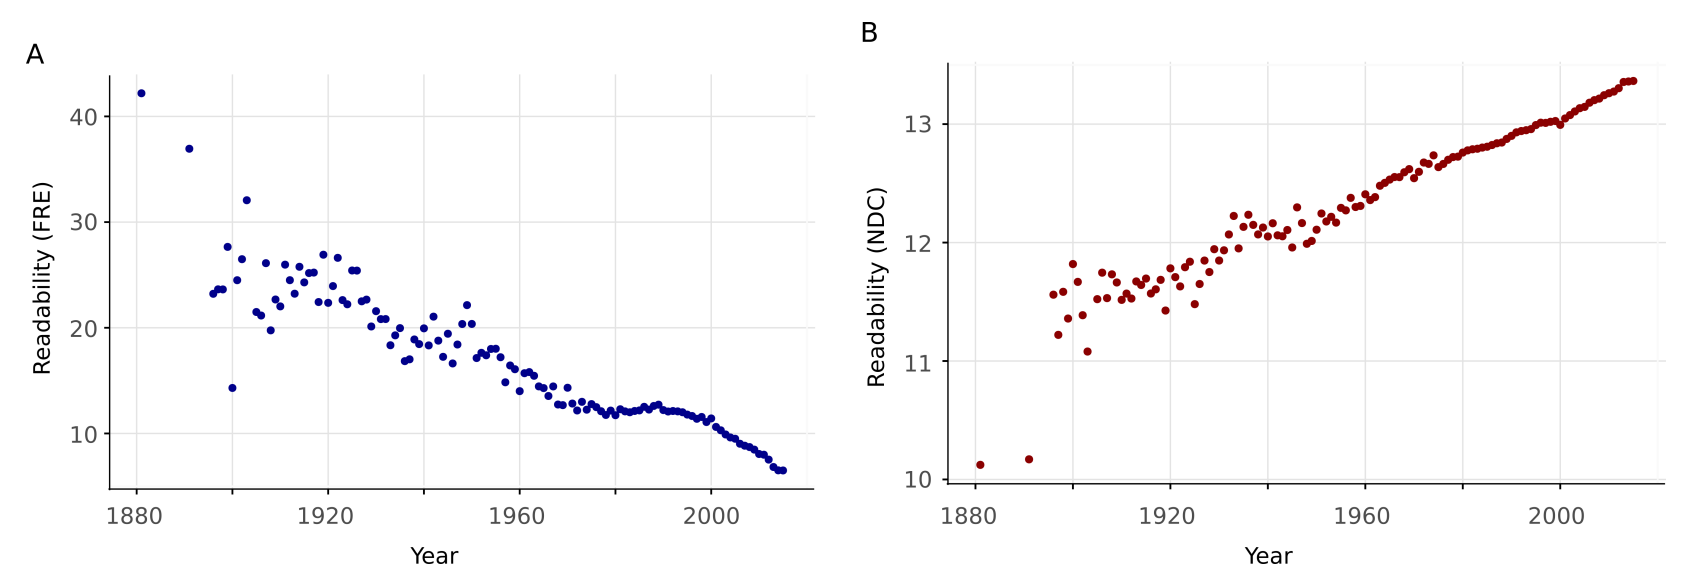
\includegraphics[width=\linewidth]{img/fre-ndc.png}
	\caption{Afbeelding uit \textcite{PlavenSigray2017}}
	\label{img:fre-ndc}
\end{figure}

De hoge leesgraad van wetenschappelijke artikelen beperkt volgens \textcite{PlavenSigray2017} twee aspecten: de toegankelijkheid en de herproduceerbaarheid.

\subsubsection{Toegankelijkheid}




Onbegrijpelijke en ontoegankelijke zinsstructuren hinderen ook vakexperten. Zo toonde onderzoek van \textcite{McNutt2014} aan dat begrip van de methodologie en resultaten cruciaal is in het kader van reproduceerbaarheid; enkel zo kunnen wetenschappers op correcte wijze een studie reproduceren en wetenschappelijke inzichten bevestigen of met verdere resultaten verrijken. Experimenten van \textcite{Hubbard2017} wijzen namelijk uit dat het net vooral de methodologie en resultaten van een wetenschappelijk artikel zijn die een hoge leesgraad vergen. In deze context is ook het onderzoek van \textcite{Hartley1999} en \textcite{Snow2010} relevant waarin ze aantonen dat het herschrijven van abstracts de begrijpbaarheid ervan kan verhogen.



% Het lezen van deze artikelen brengt uitdagingen met zich mee vanwege de syntax- en woordenschatverschillen ten opzichte van ander inzetbaar leesmateriaal in het onderwijs, waaronder nieuwsartikelen. Docenten kunnen dit aanpakken in de derde graad van het middelbaar onderwijs door te benadrukken wat de specifieke kenmerken van wetenschappelijke artikelen zijn. 

\section{Aanpakken voor geautomatiseerde tekstvereenvoudiging}

% TODO ;;;;;


\subsection{Bewezen effecten van manuele tekstvereenvoudiging -en aanpassing bij scholieren met dyslexie}

Een ondersteunende toepassing moet met een individuele analyse van de specifieke behoeften en uitdagingen van elke leerling in gedachten worden ontworpen \autocite{Gooding2022}. Instructies moeten op een begrijpelijke en geïndividualiseerde manier worden gepresenteerd om de leerlingen te helpen bij het begrijpen en toepassen van de informatie. Het is belangrijk om te erkennen dat dyslexie zich bij verschillende kinderen op verschillende manieren kan uiten. Een bijkomende stoornis heeft bijvoorbeeld geen impact op de spellingprestaties van een kind. Het is daarom belangrijk om een toepassing te ontwerpen met de diversiteit van dyslexie in het achterhoofd.

% TODO expliciet verwijzen in de tekst --> relevant voor anders

\begin{figure}[H]
	\begin{center}
		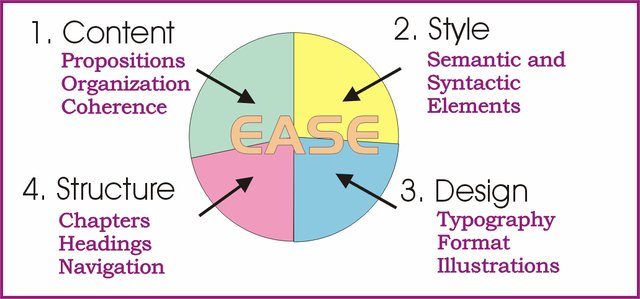
\includegraphics[width=9cm]{img/text-simplification-reading-ease.png}
	\end{center}
	\caption{Afbeelding van \textcite{Dubay2004}}
	\label{img:reading-ease}
\end{figure}


\subsection{Bewezen effecten van geautomatiseerde tekstvereenvoudiging -en aanpssing bij scholieren met dyslexie}